\documentclass[a4paper,10pt,twoside]{report}
\usepackage{geometry}\geometry{a4paper,top=3.5cm,bottom=3.5cm,%
left=2.5cm,right=2.5cm,heightrounded,bindingoffset=0mm}
\usepackage[T1]{fontenc}
\usepackage[utf8]{inputenc}
\usepackage[italian]{babel}
\usepackage{graphicx}
\usepackage[export]{adjustbox}%Per il Frame attrono le immagini e il valign
\usepackage{subfig}
\usepackage{amsmath,amsfonts,amssymb,braket,mathrsfs}
\usepackage{float}
\usepackage{tabularx,booktabs}
\usepackage{hyperref}
\usepackage{epsfig}
\usepackage{pdfpages} %Per gli allegati
%\usepackage{minipage}
\usepackage[output-decimal-marker={,}]{siunitx}
\DeclareSIUnit \days {gg}
%ILe tre righe sotto ervono per mettere il grassetto dentro la tabelle siunitex usando \B, il rosso usando \RED, e il verde usando \GREEN
\sisetup{detect-weight,mode=text}
\usepackage{etoolbox}
\newrobustcmd\B{\DeclareFontSeriesDefault[rm]{bf}{b}\bfseries}
\newrobustcmd\RED{\DeclareFontSeriesDefault[rm]{bf}{b}\color{red}}
\newrobustcmd\GREEN{\DeclareFontSeriesDefault[rm]{bf}{b}\color{myGreen}}
%%
\usepackage{tikz}
\usepackage{pgfplots,pgfplotstable}
%\pgfplotsset{compat=1.15} %indica la versione da utilizzare per pgfplot
\usetikzlibrary{patterns} % per il tratteggio
\usepgfplotslibrary{groupplots}
\pgfplotsset{compat=newest}
%\usepackage{stanli}
\usepackage{xspace}% per lo spazio intelligente
\newcommand{\e}{\`E\xspace}  %E'
\usepackage{titlesec} % per formato custom dei titoli dei capitoli
%\usepackage{sideways}%%%
% redefinizione del formato del titolo del capitolo
      % da formato
      %   Capitolo X
      %   Titolo capitolo
      %   a formato
      %      Titolo capitolo 
	\titleformat{\chapter}
        {\normalfont\Huge\bfseries}{}{0em}{}
	\titlespacing*{\chapter}{0pt}{0in}{0.02in}
	\titlespacing*{\section}{0pt}{0.2in}{0.02in}
	\titlespacing*{\subsection}{0pt}{0.10in}{0.02in}
%serve per la didascalia di tabelle e figure:
\usepackage{caption}
\captionsetup{tableposition=top,figureposition=bottom,font=small}\captionsetup{format=hang,labelfont={bf,color=pantone186}} %didascalie a più righe allineate e il nome in grassetto
%non viene allineato a sinistra se la didascalia è corta una sola riga. PERCHé??
\usepackage{xcolor}
%serve per mettere il codice con lo sfondo grigio chiaro
\definecolor{pantone186}{RGB}{206, 17, 38} %il colore del logo UNITN
\definecolor{myGray}{gray}{0.5} %più basso più scuro è
\definecolor{myGreen}{rgb}{0.0, 0.5, 0.0}
\usepackage{listings} 
\lstset{basicstyle=\small\ttfamily,
backgroundcolor=\color{black!10},%
boxpos=c,%
stringstyle=\itshape,		
lineskip=3pt,%
numbers=left,
numberstyle=\footnotesize,}
\usepackage{lscape}
\usepackage{multirow}
\usepackage{import}
\usepackage{pythontex}
\begin{document}
\pagestyle{plain}
\thispagestyle{empty}
\begin{center}
  \begin{figure}[H]
    \centerline{
\psfig{file=IMG/logo_unitn_black_centerNEW.eps,
                        width=0.8\textwidth,trim = 0 0.9cm 0 0.5cm}}
  \end{figure}
\textcolor{pantone186}{\noindent\rule{\textwidth}{.5pt}}

  \Large\textsc{Dipartimento di Ingegneria Civile, Ambientale e Meccanica\\}
  \Large{Corso di Laurea Magistrale in Ingegneria Civile
  }

  \vspace{3.7 cm} 
  %\Large\textsc{Elaborato finale\\} 
  %\vspace{1 cm} 
  \Huge\textsc{Relazione Costruzioni in Legno\\}
  
  \vspace{0.2 cm}
  \Large{\it{Rete di drenaggio acque meteoriche\\
  Quartiere “Le Albere” – Ex Parco Michelin  (Trento)}}


  \vspace{4 cm} 
  \begin{tabular*}{\textwidth}{ l @{\extracolsep{\fill}} r }
  \Large\textsc{Docenti} & \Large\textsc{Studenti}\\
  \Large{Alberto Bellin}& \Large{Nicola Meoli 225077}\\
  \Large{Maria Grazia Zanoni}& \Large{Luca Zorzi 227085}\\
  
  	
  	
  \end{tabular*}

  \vspace{3.1cm} 
  \textcolor{pantone186}{\noindent\rule{\textwidth}{1pt}}
    
  \Large{Anno accademico 2020/21}
  
\end{center}


\tableofcontents
%\setcounter{page}{1}
%Tabelle e figure sulla stessa pagina:
%Le aggiunge all'indice. phantomsection serve per non far casini con hyperref
\clearpage
\begingroup
   %\let\cleardoublepage\relax  % book
    \let\clearpage\relax        % report
        \listoftables
        \phantomsection
        \addcontentsline{toc}{chapter}{Elenco delle tabelle}
\endgroup
        %
        \clearpage
\begingroup
        \let\clearpage\relax
        \listoffigures
        \phantomsection
        \addcontentsline{toc}{chapter}{Elenco delle figure}
\endgroup
%
%%%%%%%%%%
%Comandi aggiunti:
%%%%%%%%%%
\newcommand{\red}[1]{\textcolor{pantone186}{#1}}
%

\chapter{Introduzione}
\section{Premessa}


\input{CHAPTERS/chap2_AnalisiCarichi.tex}
\chapter{Verifica degli elementi}
\section{Arcarecci}

\begin{pythontexcustomcode}{py}
import numpy as np
from StrengthClasses.glulam_strength_classes import glulam
def verifica(a,b,name):
    if a<b:
        print('La verifica a ' + name + ' è pertanto soddisfatta')
    else:
        print('La verifica a ' + name + ' non è soddisfatta')
\end{pythontexcustomcode}

\begin{pycode}[arcarecci]
glulam_class = 'GL28h'
kmod = 0.9
gammaM = 1.45
k_def = 0.6

f_mk, f_t0k, f_t90k, f_c0k, f_c90k, f_vk, f_rk, \
E0mean, E005, E90mean, E9005, Gmean, G05, Grmean, Gr05, \
rho_k, rho_mean = glulam(glulam_class)

f_md, f_t0d, f_t90d, f_c0d, f_c90d, f_vd, f_rd = (kmod * X_k / gammaM for X_k in glulam(glulam_class)[0:7])

M_d = 9.6296875 #kNm
V_d = 7.70375 #kN

M_d = M_d * 10**6 
V_d = V_d * 10**3 

b = 160
h = 200
l = 5000

###########################################################
W = b * h**2 / 6 #sezioni rettangolari
J = b*h**3 / 12

#Flessione:
sigma_md = M_d / W
f_md = kmod * f_mk / gammaM

# Sbandamento :
# Vedi pagina 291 del libro
l_t = 2500 # distanza tra due ritegni torsionali successivi (l/2)
a1 = 1.13
a2 = 1.44
az = h/2
# caso generico per il RETTANGOLO e non semplificato per h/b > 4
B = E0mean * b**3 * h / 12 # rigidezza flessionale attorno asse z
T = Gmean * b**3 * h / (3*(1 + 0.6 * b/h)) # rigidezza torsionale 
l_eff = l_t / (a1 * (1 - a2 * az/l_t * np.sqrt(B/T)))

sigma_mcrit = np.pi/l_eff * b**2 / h * E005 * np.sqrt(Gmean/E0mean)
lambda_relm = np.sqrt(f_mk/sigma_mcrit)
if lambda_relm < 0.75:
    k_crit = 1
elif lambda_relm < 1.14:
    k_crit = 1.56 - .75*lambda_relm
else:
    k_crit = 1/(lambda_relm**2)


#Taglio    
#kcrit legno lamellare = 2.5/f_vk -> b_eff = kcr * b
b_eff = 2.5/f_vk * b
tau_d = V_d * 1.5 / (b_eff * h)
f_vd = kmod * f_vk / gammaM

#Freccia
chi = 1.2
def w_inst(q): 
    w_inst_M = 5/384 * q * l**4 / (E0mean * J)
    w_inst_V = chi * 1/8 * q * l**2 / (Gmean * b * h)
    w_inst = w_inst_M + w_inst_V
    
    return w_inst

\end{pycode}

\begin{pysub}[arcarecci]
Dati di progetto per il legno lamellare $GL28h$, $\gamma_M = !{gammaM}$:
\begin{table}[H]
    \centering
    \caption{Azioni di progetto nei punti di sezione indicati in figura per la trave a doppia rastremazione}
    \begin{tabular}{c  S[table-format=4.1] S[table-format=4.3] S[table-format=3.3]}
        \toprule
		%\multicolumn{4}{c}{Azioni di progetto nei punti di sezione}\\
        Sezione & \multicolumn{1}{c}{$x$ [\si{\milli\metre}]} & \multicolumn{1}{c}{$M_d$ [\si{\kilo\newton\metre}]}& \multicolumn{1}{c}{$V_d$ [\si{\kilo\newton}]} \\
        \midrule
        A & 0. 0               & 0.0                      & !{round(V_d/10**3,3)}   \\
        B & !{round(l/2,1)}    & !{round(M_d/10**6,3)}    & 0.0						\\
        \bottomrule
    \end{tabular}
\end{table} 
\begin{table}[H]
    \centering
    \caption{Valori di progetto per la verifica della trave a doppia rastremazione}
    \begin{tabular}{lS[table-format=2.1] @{\hspace{2cm}} lS[table-format=2.3]@{\hspace{2cm}} lS[table-format=5.1]}
        \toprule
		\multicolumn{6}{c}{Valori geometrici e coefficienti di esposizione o durata del carico}\\
        \midrule
		$b$      & \SI{!{b}}{\milli\metre}     & $h$        & \SI{!{h}}{\milli\metre}   & $l$           & \SI{!{l}}{\milli\metre}  \\ 
        $\gamma_M$      & \SI{!{gammaM}}{}     & $k_{mod}$        & \SI{!{kmod}}{}   & $k_{def}$ & \SI{!{k_def}}{} \\
        \midrule
        \multicolumn{6}{c}{Valori di resistenza GL28h [\si{\mega\pascal}] } \\
        \midrule
        $f_{m,k}$    & !{f_mk}   & $f_{m,d}$    & !{round(f_md,3)}  & $E_{0,mean}$ & !{E0mean} \\
        $f_{v,k}$    & !{f_vk}   & $f_{v,d}$    & !{round(f_vd,3)}  & $E_{0,05}$   & !{E005} \\
        $f_{c,90,k}$ & !{f_c90k} & $f_{c,90,d}$ & !{round(f_c90d,3)} & $G_{mean}$   & !{Gmean} \\
        $f_{t,90,k}$ & !{f_t90k} & $f_{t,90,d}$ & !{round(f_t90d,3)} &  $G_{05}$     & !{G05}\\
        \bottomrule
    \end{tabular}
\end{table} 
Sezione di verifica: $\SI{!{b}}{} \times \SI{!{h}}{\milli\metre}$

Classe di servizio 2: $k_{mod} = !{kmod}$


disegno, momento, taglio, sezione, ecc
\subsection{Flessione}
\begin{equation} 
    \sigma_{m,d} \leq f_{m,d} = \SI{!{round(f_md,3)}}{\mega\pascal}
\end{equation}

La sollecitazione massima la si ha in mezzeria, pertanto è pari, avendo sezione rettangolare, a:
\[
\sigma_{m,d} 
= \frac{M_d}{W} 
= \frac{M_d}{\dfrac {b \cdot h^2}{6}} 
= \frac{\SI{!{round(M_d/10**6,3)}e6}{\newton\milli\metre}} {\dfrac {!{b} \cdot !{h}^2}{6} \si{\milli\metre\tothe{3}}} 
= \SI{!{round(sigma_md,3)}}{\mega\pascal} 
\]


Sebbene lo sbandamento sia impedito, pur tenendone conto si ha:
\begin{equation}
     \sigma_{m,d} \leq k_{crit} \cdot f_{m,d} 
\end{equation}
dove 
\begin{equation}
    k_{crit} =
    \begin{cases}
        1 & \text{se \quad $ \lambda_{rel,m} \leq 0.75$} \\
        1.56 - 0.75 \cdot \lambda_{rel,m} & \text{se \quad $0.75 \leq \lambda_{rel,m} \leq 1.4$} \\
        \dfrac{1}{\lambda_{rel,m}^2} & \text{se \quad $\lambda_{rel,m} \geq 0.75$}
    \end{cases}
    \quad =  !{k_crit}
\end{equation}
in cui 
\[
\begin{split}
    \lambda_{rel,m} 
    &= \sqrt{  \frac{f_{m,k}}     {\sigma_{m,crit}}          } 
    = \sqrt{  \frac{!{f_mk}}     {!{round(sigma_mcrit,1)}}  } 
    = !{round(lambda_relm,3)} \\
    \sigma_{m,crit} 
    &= \dfrac{\pi}{l_{eff}} \dfrac{b^2}{h} E_{0.05} \sqrt{\dfrac{G_{mean}}{E_{mean}}} 
    = \dfrac{\pi}{!{round(l_eff,1)}} \dfrac{!{b}^2}{!{h}} !{E005} \sqrt{\dfrac{!{Gmean}}{!{E0mean}}} 
    = \SI{!{round(sigma_mcrit,1)}}{\mega\pascal} \\
    l_{eff}  
    &= \frac{l_t}{a_1 \left(1 - a_2  \dfrac{a_z}{l_t} \sqrt{\dfrac{B}{T}}\right)} 
    = \frac{!{l_t}}{!{a1} \left(1 - !{a2}  \dfrac{!{az}}{!{l_t}} \sqrt{\dfrac{!{round(B,1)}}{!{round(T,1)}}}\right)}
    =   
    \SI{!{round(l_eff,1)}}{\milli\metre}
\end{split}
\]
avendo preso $l_t = \dfrac{l}{2}, a_z = \dfrac{h}{2}$, i coefficienti di ribaltamento $a_1, a_2$ in base alla condizione di vincolo (tabella E.2 DIN 1052:2004) ed essendo $B$ e $T$ rispettivamente la rigidezza flessionale attorno all'asse $z$ e torsionale di un rettangolo.

Quindi la resistenza di progetto vale
\[
    k_{crit} \cdot f_{m,d} 
    = k_{crit} \cdot f_{m,d}
    = !{k_crit} \cdot \SI{!{round(f_md,3)}}{\mega\pascal}
    = \SI{!{round(k_crit * f_md,3)}}{\mega\pascal}
\]
%\pyc{verifica(sigma_md,k_crit * f_md,'flessione')}

\subsection{Taglio}
Si deve avere
\begin{equation}
    \tau_d \leq f_{v,d}   
\end{equation}
La sollecitazione massima che si ha agli appoggi vale
\[
\tau_d 
= 1.5 \frac{V_d}{b_{eff} \cdot h} 
= \frac{\SI{!{round(V_d/10**3,3)}e3}{\newton}} {!{round(b_eff,1)} \cdot !{h} \si{\milli\metre\tothe{2}}} 
= \SI{!{round(tau_d,3)}}{\mega\pascal} 
\]
in cui da normativa (C.4.4.8.1.9) per il legno lamellare 
\[
    b_{eff} 
    = k_{cr} \cdot b 
    = \dfrac{2.5}{f_{v,k}} \cdot b 
    = \dfrac{2.5}{!{f_vk}} \cdot !{b}
    = \SI{!{round(b_eff,1)}}{\milli\metre}
\]
Essendo $\SI{!{round(tau_d,3)}}{\mega\pascal} < \SI{!{round(f_vd,3)}}{\mega\pascal}$ la verifica è soddisfatta.

\subsection{Freccia}
La freccia dovuta al contributo del momento flettente e del taglio, nel caso di semplice appoggio vale
\begin{equation}
    w(q) = \dfrac{5}{384} \frac{q \cdot l^4}{E_{0,mean} \cdot J} + \chi \dfrac{1}{8} \frac{q \cdot l^2}{G_{mean} \cdot b \cdot h}
\end{equation}
che, per un carico unitario e per una sezione rettangolare, assume il valore di riferimento
\begin{equation}
    w(q = \SI{1}{\kilo\newton\per\metre}) 
    = \dfrac{5}{384} \frac{1 \cdot !{l}^4}{!{E0mean} \cdot \SI{!{round(J/10**6,3)}e6}{}} + !{chi} \dfrac{1}{8} \frac{1 \cdot !{l}^2}{!{Gmean} \cdot !{b} \cdot !{h}} 
    = \SI{!{round(w_inst(1),3)}}{\milli\metre}
\end{equation}

\end{pysub}

\begin{pycode}[viti]
d = 6 # mm
d1 = 3.8 # mm
n = 2 #numero di viti
#l = 220 # mm 
f_uk = 600 # Mpa
gamma_M1 = 1.05
gamma_M2 = 1.25 # acciao. tabella 4.2 vii ntc
gammaM = 1.5 #connessione in legno 
kmod = 0.9

rho_k1 = 425
rho_k2 = 425

l_ef1 = 80
l_ef2 = 80

V_d = 7704 # N
alpha = 45 # gradi
alpha_fib1 = 90
alpha_fib2 = 45

alpha = np.radians(alpha)


#sistemare per altri angoli!
F_comp = F_traz = V_d * np.cos(alpha)

#################################################

# Verifica A)
A_res = np.pi * d1 **2 / 4
f_ax_rk_vite = 0.9 * A_res * f_uk 
f_ax_rd_vite = f_ax_rk_vite/gamma_M2

# Verifica B)
n_ef = 1 # n**0.9 
f_ax_k_1 = 0.52 * d**-0.5 * l_ef1 **-0.1 * rho_k2**0.8
k_d = min(d/8, 1)

F_ax_rk_1 = (n_ef * f_ax_k_1 * d * l_ef1 * k_d) / (1.2 * np.cos(np.radians(alpha_fib1))**2 + np.sin(np.radians(alpha_fib1))**2)
F_ax_rd_1 = F_ax_rk_1/gammaM * kmod

# Verifica C)
n_ef = 1 # n**0.9 
f_ax_k_2 = 0.52 * d**-0.5 * l_ef2 **-0.1 * rho_k1**0.8
k_d = min(d/8, 1)

F_ax_rk_2 = (n_ef * f_ax_k_2 * d * l_ef2 * k_d) / (1.2 * np.cos(np.radians(alpha_fib2))**2 + np.sin(np.radians(alpha_fib2))**2)
F_ax_rd_2 = F_ax_rk_2/gammaM * kmod

#Verifica D)
N_pl_k = np.pi * d1**2 / 4 * f_uk

c_h = (0.19 + 0.012*d)*rho_k2*((90 + alpha_fib2) / 180)
E_s = 210000
I_s = np.pi * d1**4 / 64
N_ki_k = np.sqrt(c_h * E_s * I_s)

lambda_k = np.sqrt(N_pl_k / N_ki_k)

k = 0.5 * (1 + 0.49*(lambda_k-0.2) + lambda_k**2)
k_c = 1 / (k + np.sqrt(k**2 - lambda_k**2)) if lambda_k > 0.2 else  1

F_ax_rk_buck = N_pl_k * k_c
F_ax_rd_buck = F_ax_rk_buck / gamma_M1
\end{pycode}
%%%%%%%%%%%%%%%%%%%%%
\section{Viti inclinate trave a doppia rastremazione e arcarecci}
\begin{figure}[H]
    \centering
    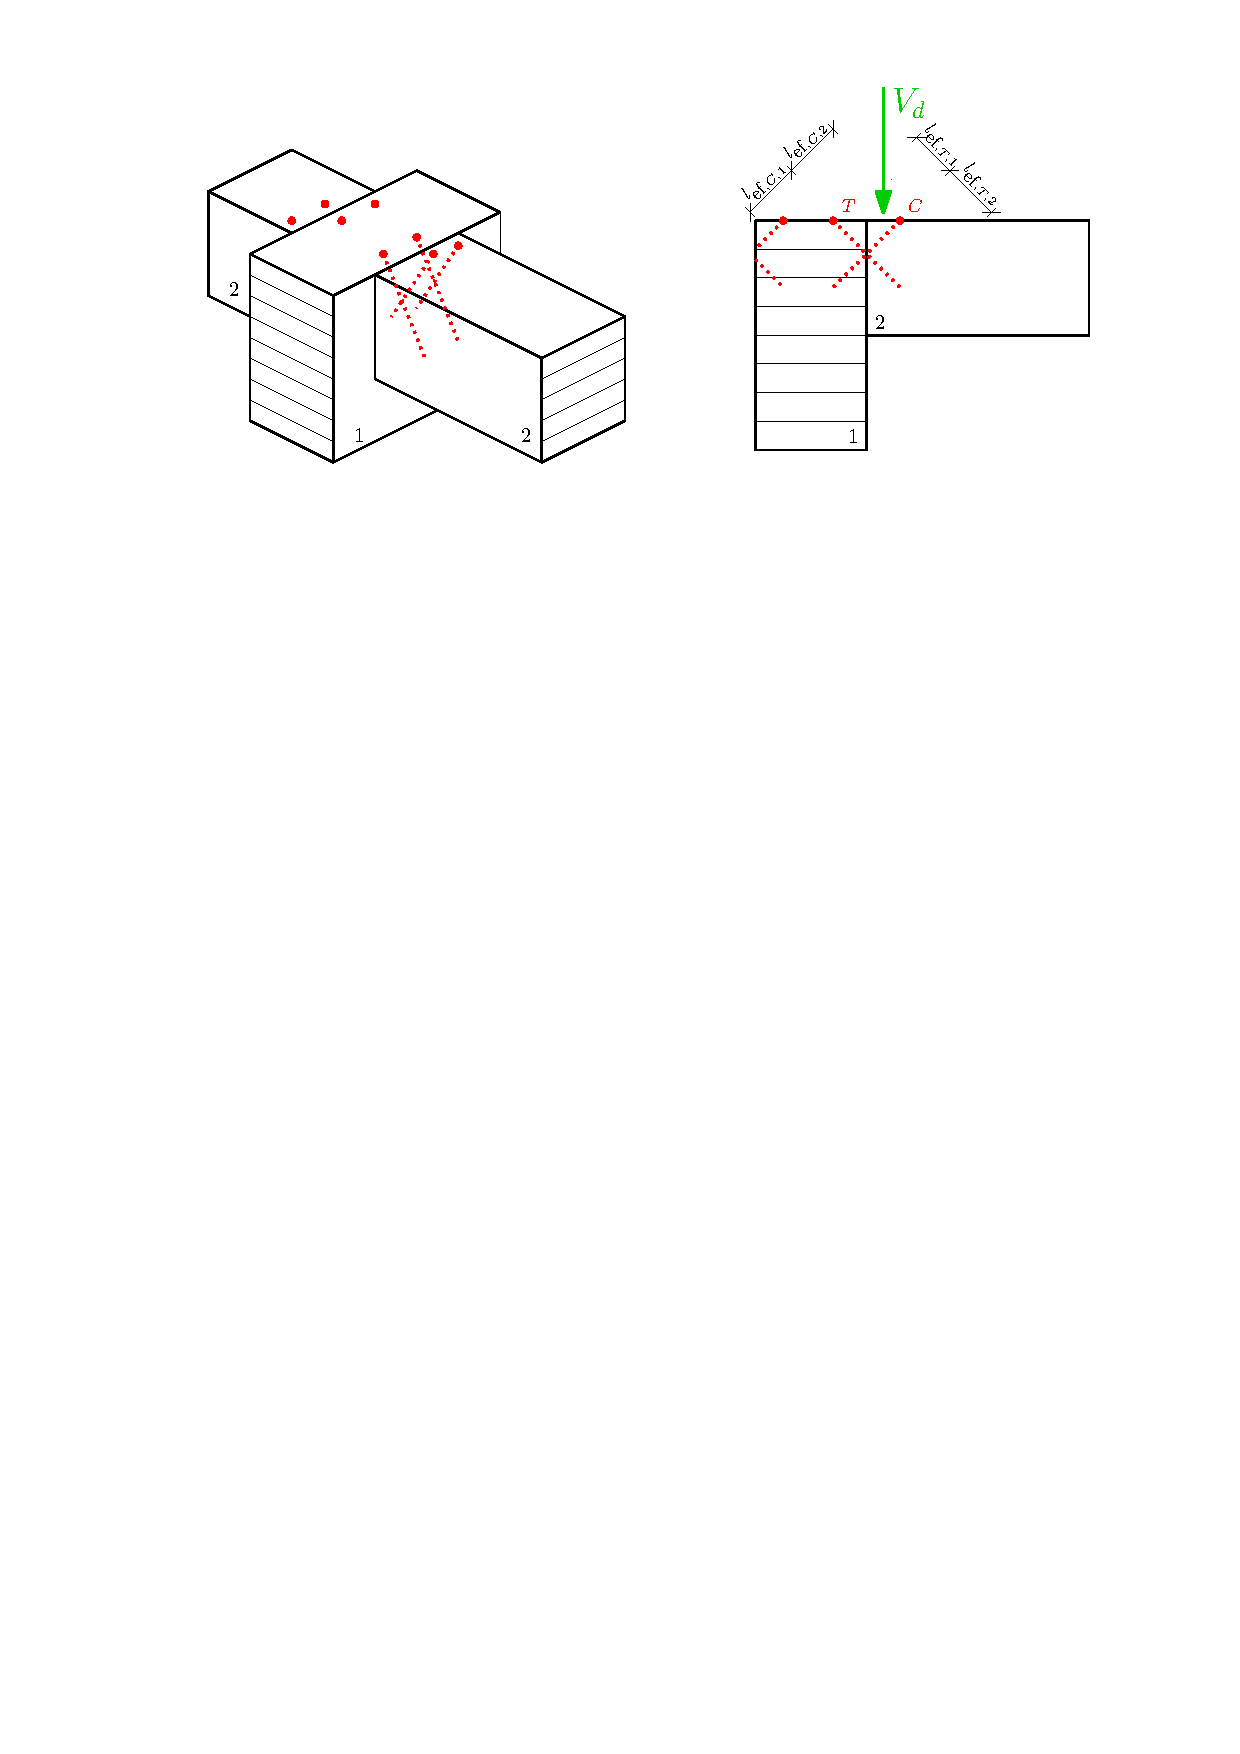
\includegraphics[]{IMG/VitiIncrociate_doppie.pdf}
    \caption{Schematizzazione della connessione tramite viti incrociate tra la trave rastremata e gli arcarecci}
    \label{fig:VitiIncrociate}
\end{figure}
\begin{pysub}[viti]
    \begin{table}[H]
        \centering
        \caption{Valori di progetto della connessione tramite vite inclinate}
        \begin{tabular}{lS[table-format=3.2] @{\hspace{2cm}} lS[table-format=2.2]@{\hspace{2cm}} lS[table-format=3.0]}
            \toprule
            \multicolumn{6}{c}{Valori di progetto della connessione tramite vite inclinate}\\
            \midrule
            $d$          & \SI{!{d}}{\milli\metre}                    & $d_1$        & \SI{!{d1}}{\milli\metre}    & $n$                     & !{n} \\
            $\rho_k^1$   & \SI{!{rho_k1}}{\kilo\gram\per\metre\cubed} & $l_{ef}^1$   & \SI{!{l_ef1}}{\milli\metre} & $\alpha_{fibre-vite}^1$ & \SI{!{alpha_fib1}}{\degree} \\
            $\rho_k^2$   & \SI{!{rho_k2}}{\kilo\gram\per\metre\cubed} & $l_{ef}^2$   & \SI{!{l_ef2}}{\milli\metre} & $\alpha_{fibre-vite}^2$ & \SI{!{alpha_fib2}}{\degree} \\
            $\gamma_M$   & !{gammaM}                                  & $k_{mod}$    & !{kmod}                     &                         & \\
            $\gamma_{M1}$  & !{gamma_M1}                                & $\gamma_{M2}$  & !{gamma_M2}                 & $f_{u,k}$               & \SI{!{f_uk}}{\mega\pascal}\\
            \bottomrule
        \end{tabular}
    \end{table} 
La connessione tra la trave a doppia rastremazione e ciascun arcareccio viene eseguita tramite due viti a tutto filetto.
Entrambe le viti sono sottoggette a puro sforzo assiale ed essendo inclinate ad $\alpha = \SI{45}{\degree}$ gli sforzi valgono 
\begin{equation}
    F_{traz} = F_{comp} = V^{arcareccio} \cos(\alpha) = \SI{!{V_d}}{\newton} \cos\SI{45}{\degree} = \SI{!{round(F_comp,1)}}{\newton} \quad .
\end{equation}

Per la vite sottoposta a sola trazione si tengono conto dei modi di rottura per trazione del materiale acciaio e della rottura per estrazione della vite lato elemento principale $1$ e lato elemento secondario $2$.
Per la vite sottoposta a sola compressione si tiene conto della rottura per estrazione nei due elementi, e della rottura a instabilità per carico di punta a compressione.
Infine si tengono conto delle distanze minime dal bordo e dalle estremità.

Le vite utilizzate sono della ditta Wurth e denominate \textit{ASSY PLUS VG TC}.
\begin{figure}[H]
    \centering
    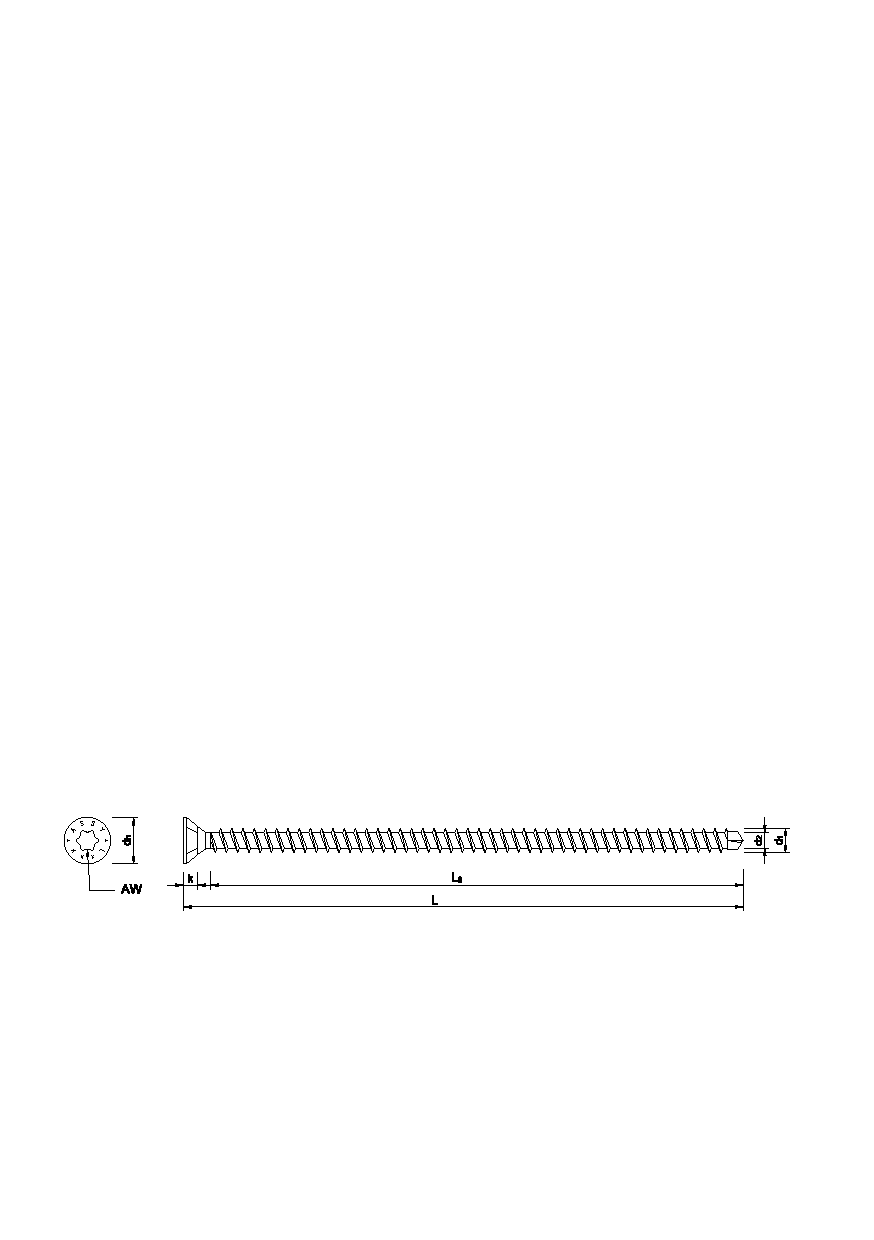
\includegraphics[width = 0.9\textwidth]{IMG/ViteWurth.pdf}
    \caption{Rappresentazione della vite ASSY PLUS VG TC nel quale la nomenclatura corrisponde a $d_1 = d$ e $d_2 = d_1$}
    \label{fig:ViteWurth}
\end{figure}
\subsection{Resistenze caratteristiche Rk del singolo connettore}
\paragraph{Rottura acciaio}
\begin{equation}
    F_{ax,Rk}^{acciaio} 
    = 0.9 \, A_{res} \, f_{u,k} 
    = 0.9 \, \dfrac{\pi d_1^2}{4} \, f_{u,k} 
    = \frac{\pi \, (\SI{!{d1}}{\milli\metre})^2}{4} \, \SI{!{f_uk}}{\mega\pascal} 
    = \SI{!{round(f_ax_rk_vite,1)}}{\newton}
\end{equation}

\paragraph{Estrazione elemento 1}
\begin{equation}
    F_{ax,Rk}^{estr. 1} %
    = \frac{f_{ax,k} \cdot d \cdot l_{ef}^i \cdot k_{d} \cdot n_{ef}}%
        {\SI{1.2}{} \cos^2 \alpha_{f-v} + \sin^2 \alpha_{f-v}} %
    = \frac{\SI{!{round(f_ax_k_1,2)}}{} \cdot !{d} \cdot !{l_ef1} \cdot !{k_d} \cdot !{n_ef}}%
        {\SI{1.2}{} \cos^2 !{alpha_fib1} + \sin^2 !{alpha_fib1}} %
    = \SI{!{round(F_ax_rk_1,1)}}{\newton} 
\end{equation}
dove
\[
    \begin{split}
        f_{ax,k} 
        &= \SI{0.52}{} \cdot d^{-0.5} \cdot l_{ef}^{-0.1, \, i} \cdot \rho_k^{0.8, \, i} 
        = \SI{0.52}{} \cdot !{d}^{-0.5} \cdot !{l_ef1}^{-0.1} \cdot !{rho_k2}^{0.8}
        = \SI{!{round(f_ax_k_1,2)}}{\mega\pascal} \\
        %
        k_{d} 
        &= \min \left( \dfrac{d}{8} ; 1 \right)
        =\min \left( \dfrac{!{d}}{8} ; 1 \right) 
        = !{k_d} \\
        %
        \alpha_{f-v}
        &= \SI{!{alpha_fib1}}{\degree} \quad \text{angolo tra la direzione delle fibre e la vite} \\
        %
        n_{ef} 
        &= n^{0.9} 
        = !{n_ef}
    \end{split}
\]

\paragraph{Estrazione elemento 2}
\begin{equation}
    F_{ax,Rk}^{estr. 2} %
    = \frac{f_{ax,k} \cdot d \cdot l_{ef}^i \cdot k_{d} \cdot n_{ef}}%
        {\SI{1.2}{} \cos^2 \alpha_{f-v} + \sin^2 \alpha_{f-v}} %
    = \frac{\SI{!{round(f_ax_k_2,2)}}{} \cdot !{d} \cdot !{l_ef2} \cdot !{k_d} \cdot !{n_ef}}%
        {\SI{1.2}{} \cos^2 !{alpha_fib2} + \sin^2 !{alpha_fib2}} %
    = \SI{!{round(F_ax_rk_2,1)}}{\newton} 
\end{equation}
dove
\[
    \begin{split}
        f_{ax,k} 
        &= \SI{0.52}{} \cdot d^{-0.5} \cdot l_{ef}^{-0.1, \, i} \cdot \rho_k^{0.8, \, i} 
        = \SI{0.52}{} \cdot !{d}^{-0.5} \cdot !{l_ef2}^{-0.1} \cdot !{rho_k1}^{0.8}
        = \SI{!{round(f_ax_k_2,2)}}{\mega\pascal} \\
        %
        k_{d} 
        &= \min \left( \dfrac{d}{8} ; 1 \right)
        =\min \left( \dfrac{!{d}}{8} ; 1 \right) 
        = !{k_d} \\
        %
        \alpha_{f-v}
        &= \SI{!{alpha_fib2}}{\degree} \\
        %
        n_{ef} 
        &= n^{0.9} 
        = !{n_ef}
    \end{split}
\]

\paragraph{Instabilità}
Le formule che seguono derivano dal documento ETA del produttore \textit{11/0190}.
\begin{equation}
    F_{ax,Rk}^{buck} = k_c \cdot N_{pl,k} = \SI{!{round(k_c,3)}}{} \cdot \SI{!{round(N_pl_k,1)}}{\newton} = \SI{!{round(F_ax_rk_buck,1)}}{\newton}
\end{equation}
dove
\[
    \begin{split}
        k_c 
        &= 
        \begin{cases}
            1 & \text{se \quad $ \overline{\lambda}_k \leq 0.2$} \\
            \dfrac{1}{k + \sqrt{k^2 - \overline{\lambda}_k^2 }} & \text{se \quad $\overline{\lambda}_k > 0.2$}
        \end{cases} 
        \quad = \SI{!{round(k_c,3)}}{} \\
        N_{pl,k}
        &= \frac{\pi \, d_1^2}{4} f_{y,k} 
        = \frac{\pi \, (\SI{!{d1}}{\milli\metre})^2}{4} \, \SI{!{f_uk}}{\mega\pascal}
        = \SI{!{round(N_pl_k,1)}}{\newton}\\
    \end{split}
\]
in cui
\[
    \begin{split}
        k 
        &= 0.5 \left[ 1 + 0.49 \left(\overline{\lambda}_k - 0.2 \right) + \overline{\lambda}_k^2 \right]
        = 0.5 \left[ 1 + 0.49 \left(!{round(lambda_k,3)} - 0.2 \right) + !{round(lambda_k,3)}^2 \right] 
        = \SI{!{round(k,4)}}{} \\
        \overline{\lambda}_k
        &= \sqrt{\frac{N_{pl,k}}{N_{ki,k}}}
        = \sqrt{\frac{\SI{!{round(N_pl_k,1)}}{\newton}}{\SI{!{round(N_ki_k,1)}}{\newton}}} 
        = \SI{!{round(lambda_k,3)}}{} \\
        N_{ki,k}
        &= \sqrt{c_h E_s I_s} 
        = \sqrt{\SI{!{round(c_h,2)}}{} \cdot \SI{!{E_s}}{} \cdot \SI{!{round(I_s,3)}}{}}
        = \SI{!{round(N_ki_k,1)}}{\newton}\\
        c_h 
        &= (0.19 + 0.012 \, d) \, \rho_k^i \dfrac{\SI{90}{\degree} + \alpha_{f-v}^i}{\SI{180}{\degree}}
        = (0.19 + 0.012 \, d) \, \SI{!{rho_k2}}{} \dfrac{90 + !{alpha_fib2}}{180} 
        = \SI{!{round(c_h,2)}}{} \\
        & \qquad\text{in cui si è preso il minore tra le due combinazioni di $\alpha_{f-v}$ e $\rho_k$}\\ 
        E_s
        &= \SI{!{E_s}}{\mega\pascal}\\
        I_s
        &= \frac{\pi \, d_1^4}{64}
        = \frac{\pi \, \SI{!{d1}}{}^4}{64}
        = \SI{!{round(I_s,3)}}{\milli\metre\tothe{4}}
    \end{split}
\]

\subsection{Resistenze di progetto Rd del singolo connettore}
\begin{align}
    F_{ax,Rd}^{acciaio} 
    &= \dfrac{F_{ax,Rk}^{acciaio}}{\gamma_{M2}} 
    = \dfrac{\SI{!{round(f_ax_rk_vite,1)}}{\newton}}{!{gamma_M2}} 
    = \SI{!{round(f_ax_rd_vite,1)}}{\newton} \label{eq:viti_a} \\
    %
    F_{ax,Rd}^{estr. 1} 
    &= \dfrac{k_{mod} \cdot F_{ax,Rk}^{estr. 1}}{\gamma_{M}} 
    = \dfrac{!{kmod} \cdot \SI{!{round(F_ax_rk_1,1)}}{\newton}}{!{gammaM}} 
    = \SI{!{round(F_ax_rd_1,1)}}{\newton} \label{eq:viti_b} \\
    %
    F_{ax,Rd}^{estr. 2} 
    &= \dfrac{k_{mod} \cdot F_{ax,Rk}^{estr. 2}}{\gamma_{M}} 
    = \dfrac{!{kmod} \cdot \SI{!{round(F_ax_rk_2,1)}}{\newton}}{!{gammaM}} 
    = \SI{!{round(F_ax_rd_2,1)}}{\newton} \label{eq:viti_c} \\
    %
    F_{ax,Rd}^{buck} 
    &= \dfrac{F_{ax,Rk}^{buck}}{\gamma_{M1}} 
    = \dfrac{\SI{!{round(F_ax_rk_buck,1)}}{\newton}}{!{gamma_M1}} 
    = \SI{!{round(F_ax_rd_buck,1)}}{\newton} \label{eq:viti_d}
\end{align}


La resistenza di progetto del singolo connettore vale,
per la sollecitazione di trazione:
\begin{equation}
    F_{ax,Rd,traz}^\textup{connettore} = \min[\text{eqq.} \, (\ref{eq:viti_a}), (\ref{eq:viti_b}), (\ref{eq:viti_c})] = \SI{!{round(min(f_ax_rd_vite,F_ax_rd_1,F_ax_rd_2),1)}}{\newton} \, ;
\end{equation}
mentre per quella di compressione:
\begin{equation}
    F_{ax,Rd,comp}^\textup{connettore} = \min[\text{eqq.} \, (\ref{eq:viti_b}), (\ref{eq:viti_c}), (\ref{eq:viti_d})] = \SI{!{round(min(F_ax_rd_1,F_ax_rd_2,F_ax_rd_buck),1)}}{\newton} \, .
\end{equation}

\subsection{Resistenza di progetto della connessione e verifica}
Avendo una doppia vite le resistenze di progetto della connessione equivalgolo alle resistenze della singola vite appena calcolate, moltiplicate per il numero efficace $n_{ef} = n^{0.9} = !{round(n**0.9,2)}$.

Per la sollecitazione di trazione si ha
\begin{equation}
    F_{ax,Rd,traz}^\textup{connessione} = \SI{!{round(n**0.9 * min(f_ax_rd_vite,F_ax_rd_1,F_ax_rd_2),1)}}{\newton} > F_{traz} = \SI{!{round(F_traz,1)}}{\newton} ;
\end{equation}
mentre per quella di compressione:
\begin{equation}
    F_{ax,Rd,comp}^\textup{connessione} = \SI{!{round(n**0.9 * min(F_ax_rd_1,F_ax_rd_2,F_ax_rd_buck),1)}}{\newton} > F_{comp} = \SI{!{round(F_comp,1)}}{\newton}
\end{equation}

Le verifiche sono pertanto soddisfatte
\subsection{Distanze minime e distanze effettive}
Secondo il paragrafo 8.7.2 le distanze minime devono essere almeno di:
\begin{equation}
    a_1 = 7d = !{7*d} \quad a_2 = 5d = !{5*d} \quad a_{1,CG} = 10d = !{10*d} \quad a_{2,CG} = 4d= \SI{!{4*d}}{\milli\metre}
\end{equation}
che sono ampiamente rispettate in quanto $a_{2,CG} + a_2 + a_2 + a_{2,CG} = \SI{!{18*d}}{\milli\metre} < \SI{160}{\milli\metre}$ 
\end{pysub}

\end{document} 